%(CC) Samo Penic, some rights reserved
%To delo avtorja je ponujeno pod Creative Commons Priznanje avtorstva- Deljenje pod enakimi pogoji 2.5 Slovenija licenco.
%
%Dokument lahko uporabite v skladu s Creative comons SA 2.5 Slovenija licenco.

\documentclass{beamer}
\usepackage{multimedia}
\usepackage[slovene]{babel}
\usepackage{beamerthemesplit}
\usepackage{graphicx}
\usepackage{amsmath}
%\usepackage{upgreek}
%\usepackage{ifpdf}
\hypersetup{pdfpagemode=FullScreen}


%\usetheme{Madrid}
\usetheme{Warsaw}
%\usetheme{Berlin}
%\usetheme{Marburg}
\title[Odprta koda]{Prosto programje in odprta koda; uvod, napovednik in definicije}
%\subtitle{}
\author{Samo Peni\v{c}\\}
\date{
\center{Delavnica v KuFE, Ljubljana 3.11.2015}
}

\setbeamercovered{dynamic}


\newcommand{\vir}[1]{\tiny{Vir: #1}}
\begin{document}

\frame{\titlepage}
%\frame{\tableofcontents}

\section{Aktualni dogodki}
\begin{frame}
\frametitle{Aktualno -- ``1984''}
\begin{itemize}
\item Kontraverzna nadgradnja na Windows 10
\item Sprejem zakona o telekomunikacijah v EU in nevtralnost interneta
\item "Zvi"zga"ci in politi"cne krize
\item Aktivisti"cno delovanje v Siriji
\item Vsesplo"sna cenzura in medijska manipulacija
\item Osebna Svoboda
\end{itemize}
\end{frame}

\section{Osnovni pojmi}

\subsection{Izvorna koda -- Source Code}
\begin{frame}
\frametitle{Kratek pregled razvoja elektronskega ra"cunalnika}
\begin{itemize}
\item 1830, Charles Babbage -- Mehanski analiti"cni stroj
\item 1936, Allan Turing -- teoreti"cne osnove
\item 1941, Karl Zuse Z3, elektromehanski ra"cunalnik
\item 1943, Colossus, prvi elektronski ra"cunalnik
\item 1946, Eniac
\item 1948, SSEM, prvi el. ra"cunalnik s programom v pomnilniku
\end{itemize}
\end{frame}

\begin{frame}
\frametitle{Manchester Small Scale Experimental Machine}
Primer delovanja preprostega procesorja

\begin{block}{Strojni ukazi}
{\tiny
\begin{tabular}{l|l|l}
Strojna koda& Ukaz& Opis\\
\hline\hline
000& JMP S& Brezpogojni skok na naslov S (abs. skok)\\
100& JRP S& Skok na naslov trenutni+S (rel. skok)\\
010& LDN S& Nalo"zi negativno vrednost iz lokacije S\\
110& STO S& Shrani akumulator na lokacijo S\\
001& SUB S& Od"stej S od akumulatorja in shrani nazaj v akumulator\\
011& CMP & Presko"ci izvajanje naslednjega ukaza, "ce je v akumulatorju neg. vrednost\\
111& STP & Ustavi izvajanje\\
\hline\hline
\end{tabular}
}
\end{block}
\begin{minipage}{0.2\linewidth}
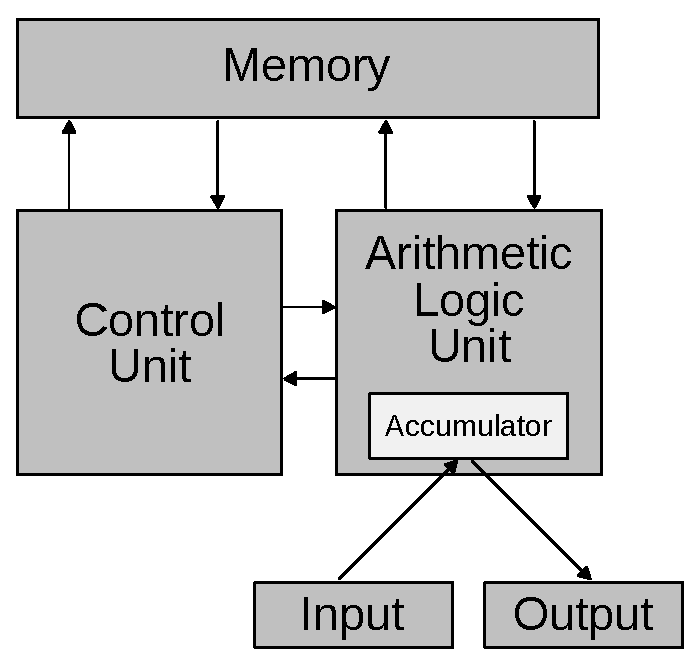
\includegraphics[width=\linewidth]{slike/Von_Neumann_architecture.pdf}
\end{minipage}%
\begin{minipage}{0.6\linewidth}
Primer: $ x+y = -(-x-y)$
\begin{center}
\texttt{LDN X}

\texttt{SUB Y}

\texttt{STO S}

\texttt{LDN S}
\end{center}
\end{minipage}
\end{frame}

%\subsection{Izvorna koda -- Source code}
\begin{frame}
\frametitle{Izvorna koda}
\begin{block}{}
Izvorna koda (angl. \textit{Source code}) je skupina navodil napisana v programskem jeziku, namenjena la"zjemu razumevanju in hitrej"semu razvoju. V sodobnih programskih jezikih je izvorna koda po navadi razdeljena v ve"c datotek. Izvorna koda ra"cunalni"skega programa je skupek datotek, ki jih ra"cunalnik prevede v strojno kodo. Izvorna koda se lahko prevede s pomo"cjo prevajalnika v strojno kodo pred razpo"siljanjem ali pa uporabni"ski ra"cunalnik program sam prevede v bitno kodo (bytecode) s pomo"cjo prevajalnika JIT.
\end{block}
\hfill\vir{Wikipedia}
\end{frame}

\begin{frame}
\frametitle{Izvorna koda in strojna koda}
\begin{center}
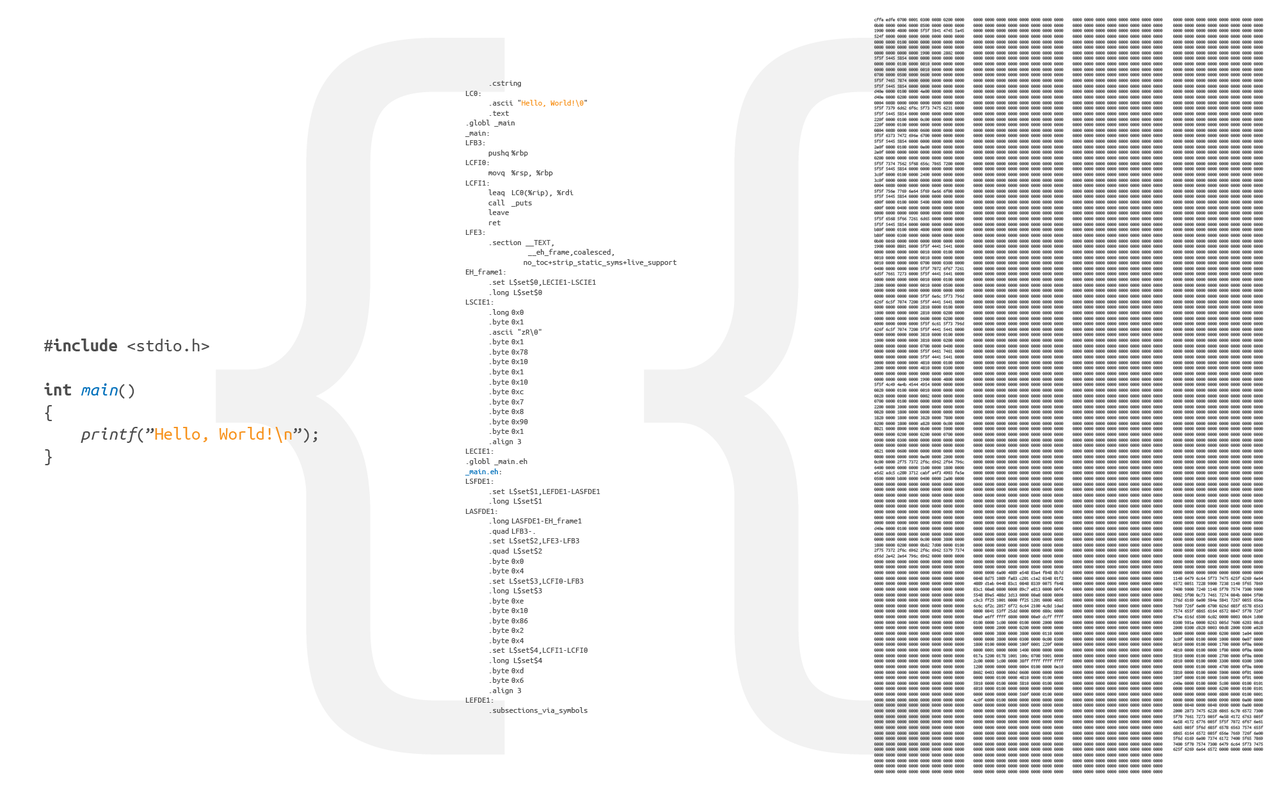
\includegraphics[width=\linewidth]{slike/source_code.png}
\end{center}
\vir{http://ntvespkr.tumblr.com/}
\end{frame}

\subsection{Heker -- Hacker}
\begin{frame}
\frametitle{Heker, angl. hacker}
\begin{block}{}
\begin{center}
Heker je ra"cunalni"ski znalec, entuziast.
\end{center}
\end{block}
\end{frame}
\begin{frame}
\frametitle{Heker -- definicija iz \textit{Jargon file} slovarja}
\begin{enumerate}
\item oseba, ki jo veseli raziskovanje detajlov programabilnih sistemov in rada raziskuje kako jih raz"siriti
\item nekdo, ki entuziasti"cno programira oz. u"ziva ob programiranju, ne samo ob ``teoretiziranju''
\item ekspertni uporabnik nekega programa (recimo ``unix heker'')
\item ekspert "cesarkoli
\item nekdo, ki ga veselijo intelektualni izzivi oz. kreativno premagovanje ovir in re"sevanje problemov
\item (zastarelo) zlonameren posameznik, ki posku"sa pridobiti informacije z bolj ali manj naklju"cnimi operacijami. Sedaj je uveljaven izraz za tak"snega posameznika kreker -- angl. Cracker
\end{enumerate}
\end{frame}


\section{Razvoj gibanja prostega programja in odprte kode}

\subsection{MIT AI Labs}
\begin{frame}
\frametitle{Za"cetki hekerske kulture}
\begin{itemize}
\item Programska oprema do srednjih 70-ih let ni bila komercialno zanimiva
\item Programsko opremo vzr"zujejo ve"cinoma hekerji -- med njimi velja nenapisan dogovor deljenja izvorne kode
\item Jabolko spora v MIT AI laboratories -- prototipni laserski tiskalnik
\item Leta 1980 na prizori"s"ce stopi Richard Matthews Stallman, ki ostaja borec za prosto programje "se danes
\end{itemize}
\end{frame}

\begin{frame}
\frametitle{Richard M. Stallman}
\begin{center}
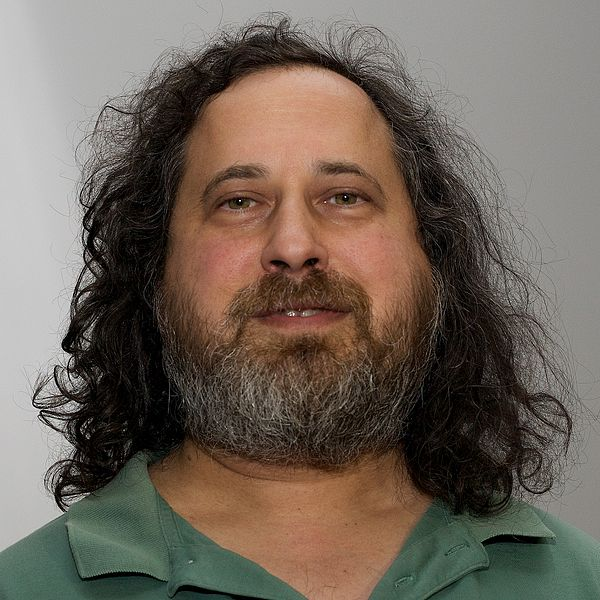
\includegraphics[width=0.5\linewidth]{slike/RMS.jpg}
\end{center}
\vir{commons.wikimedia.org (slika iz leta 2008)}
\end{frame}


\subsection{Izdajstvo hekerskega kodeksa}
\begin{frame}
\frametitle{Izdajstvo hekerskega kodeksa}
\begin{itemize}
\item Brian Reid leta 1979 ponudi svoj program \textit{Scribe} s "casovno bombo (danes: \textit{Shareware})
\item Richard Greenblatt iz MIT AIL naredi podjetje \textit{Lisp Machine Inc.}
\item Iz MIT AIL nastane spin-off podjetje \textit{Symbolics}. Vodi ga Russ Nofster. Znani heker Bill Gosper. Stallman jih ``forka''.
\item Neznani profesor iz Carnegie Mellon University (gonilniki za tiskalnik!)
\end{itemize}
\end{frame}

\begin{frame}
\frametitle{Odprto pismo ra"cunalni"skim navdu"sencem}
\begin{center}
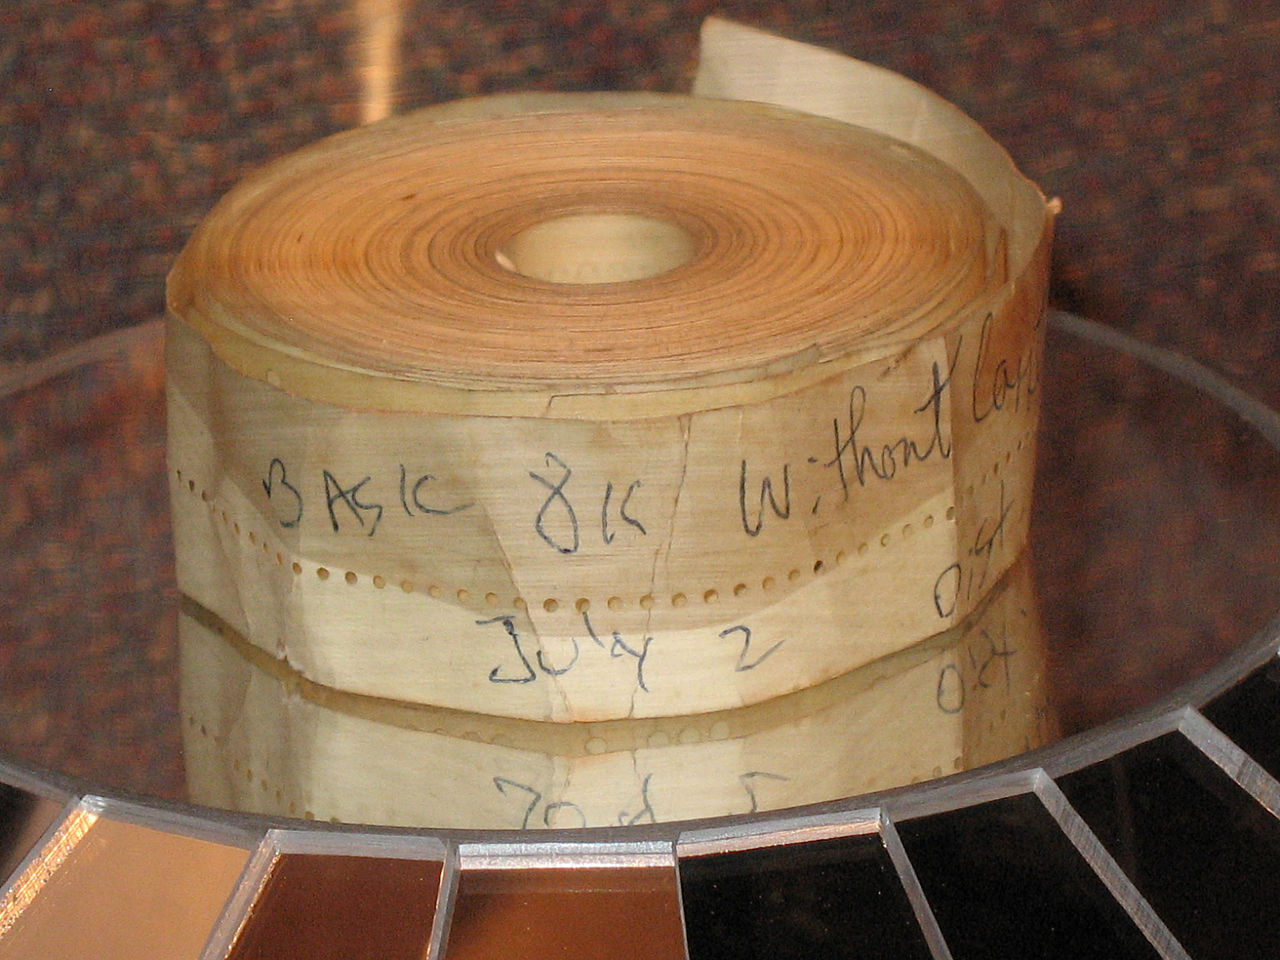
\includegraphics[width=0.6\linewidth]{slike/Altair_BASIC_Paper_Tape.jpg}
\end{center}
\end{frame}

\subsection{Gnu Project in FSF}
\begin{frame}
\begin{block}{Software wants to be free}
``Software users should have the freedom to share and to be able to study and make changes to the software that they use. Attempts by proprietary software vendors to prohibit these acts are antisocial and unethical.''

\hfill\tiny Richard M. Stallman
\end{block}
\end{frame}
\begin{frame}
\frametitle{Free Software Foundation}
\begin{itemize}
\item Septembra 1983 RMS ustanovi GNU project z namenom ustvariti prosti operacijski sitem
\item 1985 GNU Manifesto in ustanovitev neprofitne organizacije \textit{Free software foundation}
\item 1989 Prvi ra"cunalni"ski program pod licenco GPL (\textit{GNU Public Licence})
\item Z ekipo RMS razvije Emacs, GCC, GDB, gmake, ...
\item 1990 RMS in ekipa za"cnejo razvijati jedro operacijskega sistema \textit{GNU Hurd}
\end{itemize}
\end{frame}

\subsection{Linux}
\begin{frame}
\frametitle{Elektronska po"sta iz finske}
\begin{block}{}
\tiny
From: mailto: torvalds@klaava.Helsinki.Fi (Linus Benedict Torvalds)\\
\vskip0.2cm

To: Newsgroups: comp.os.inix\\
Subject: What would you like to see most in minix?\\
Summary: small poll for my new operating system\\
Message-ID: <mailto: 1991Aug25.205708.9541@klaava.Helsinki.Fi\\
Hello everybody out there using minix — I’m doing a (free) operating\\
system (just a hobby, won’t be big and professional like gnu) for 386\\
(486) AT clones. This has been brewing since april, and is starting to\\
get ready. I’d like any feedback on things people like/dislike in\\
minix, as my OS resembles it somewhat (same physical layout of the\\
file-system (due to practical reasons) among other things).\\
\vskip0.2cm
I’ve currently ported bash (1.08) and gcc (1.40), and things seem to\\
work. This implies that I’ll get something practical within a few\\
months, and I’d like to know what features most people would want. Any\\
suggestions are welcome, but I won’t promise I’ll implement them :-).\\
\vskip0.2cm
Linus (mailto: torvalds@klaava.helsinki.fi)\\
\vskip0.2cm
PS. Yes — it’s free of any minix code, and it has a multi-threaded fs.\\
It is NOT protable (uses 386 task switching etc), and it probably\\
never will support anything other than AT-harddisks, as that’s all I\\
have :-(.
\end{block}
\end{frame}

\begin{frame}
\frametitle{Linus Torvalds}
\begin{center}
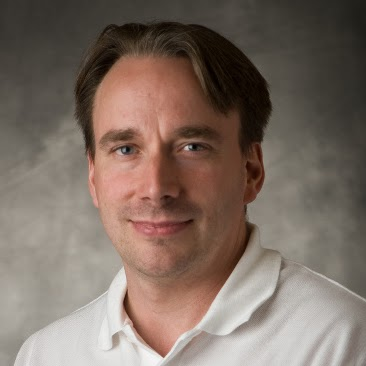
\includegraphics[width=0.5\linewidth]{slike/Linus.jpg}
\end{center}
\vir{Google+ profil Linusa Torvaldsa}
\end{frame}
\begin{frame}
\frametitle{Linux}
\begin{itemize}
\item z uporabo GNU orodij Linus zgradi jedro operacijskega sistema Linux
\item Linux je Un*xu podoben OS, kopatibilen s POSIX standardom
\item leta 1993 izda Linux pod GPL licenco.
\item 71\% programski jezik C
\item Od vgrajenih sistemov, pametnih telefonov, tablic, osebnih ra"cunalnikov, stre"znikov, superra"cunalnikov, vesoljskih postaj
\item ponavadi ga dobimo v obliki distribucije z uporabni"skimi programi
\item je prvi projekt, ki je uporabil talent programerjev celega sveta!
\end{itemize}
\end{frame}

\begin{frame}
\frametitle{Rodoslovno drevo Un*x operacijskih sistemov}
\begin{center}
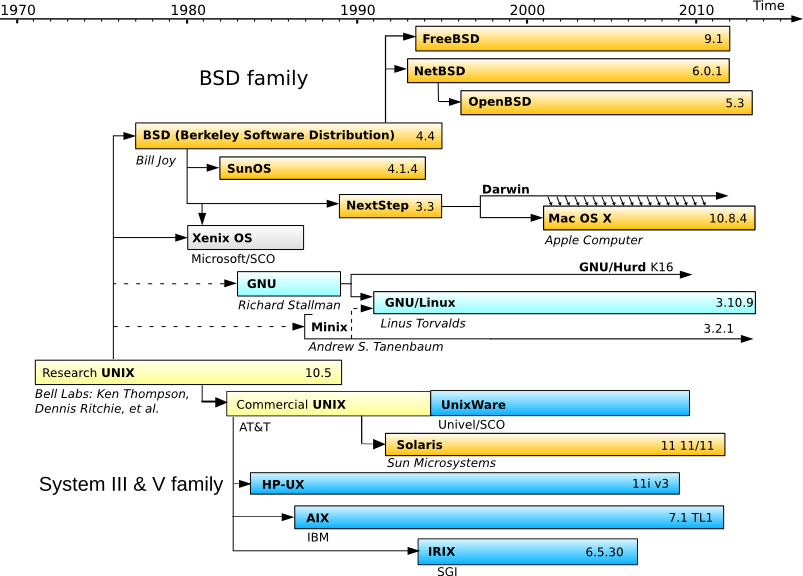
\includegraphics[width=0.75\linewidth]{slike/Unix_history.png}
\end{center}
\vir{Wikipedia}

\end{frame}

\subsection{Odprta koda}
\begin{frame}
\frametitle{Open Source Initiative}

\begin{itemize}
\item 1998 Eric S. Raymond eden izmed glavnih ustanoviteljev gibanja za Odprto kodo
\item Namen je promovirati prosto programje oz. odprto kodo v komercialne namene
\end{itemize}
\end{frame}

\begin{frame}
\frametitle{Eric S. Raymond}
\begin{center}
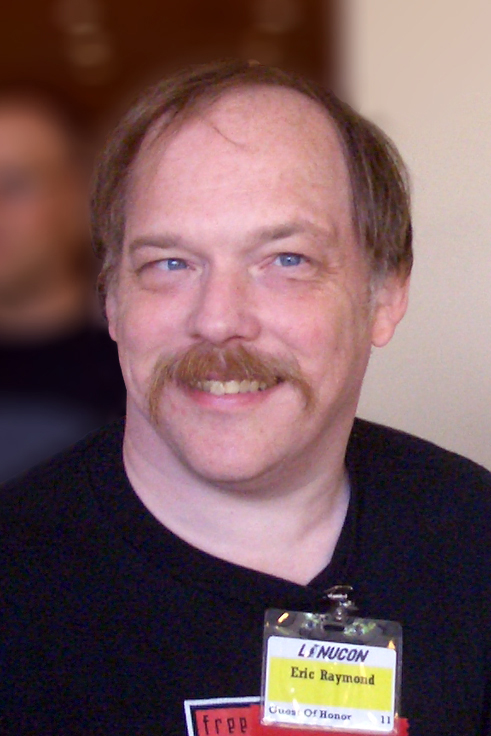
\includegraphics[width=0.35\linewidth]{slike/ESR.jpg}
\end{center}
\vir{Wikipedia}
\end{frame}

\begin{frame}
\frametitle{The Cathedral and the Bazaar}
\begin{center}
Obvezno preberi: The Cathedral and the Bazaar (avtor: ESR)
\end{center}
\end{frame}


\begin{frame}
\frametitle{FSF vs. OSI}
\tiny
\begin{columns}[l]
\column{0.5\linewidth}
FSF (4 Freedoms)
\begin{itemize}
\item Svoboda poganjanja programov za katerikoli namen
\item Svoboda preu"cevanja delovanja programa in predelave po potrebi
\item Svoboda redistribucije kopij
\item Svoboda do izbolj"save programa in objave izbolj"sav javnosti
\end{itemize}
\column{0.5\linewidth}
OSI (10 Zapovedi)
\begin{itemize}
\item Prosta redistribucija
\item Izvorna koda mora biti prilo"zena
\item Dovoljena so izpeljana dela
\item Avtor jam"ci za integriteto kode
\item Diskriminacija ljudi/skupin je prepovedana
\item Diskriminacija podro"cij uporabe je prepovedana
\item Prilo"zena mora biti licenca
\item Licenca ne sme biti posebej napisana za posamezen produkt
\item Licenca ne sme biti restriktivna do ostalega programja
\item Licenca mora biti nevtralna do tehnologije
\end{itemize}
\end{columns}
\end{frame}

\begin{frame}
\frametitle{FSF vs. OSI (povzetek)}
\begin{block}{}
\begin{itemize}
\item FSF promovira prosto programje v smislu etike in morale
\item OSI promovira odprto kodo pragmati"cno, s fokusom na na"cinu razvoja programja in marketinga
\end{itemize}
\end{block}
\end{frame}

\subsection{Boji"s"ce odprte kode}
\begin{frame}
\begin{center}
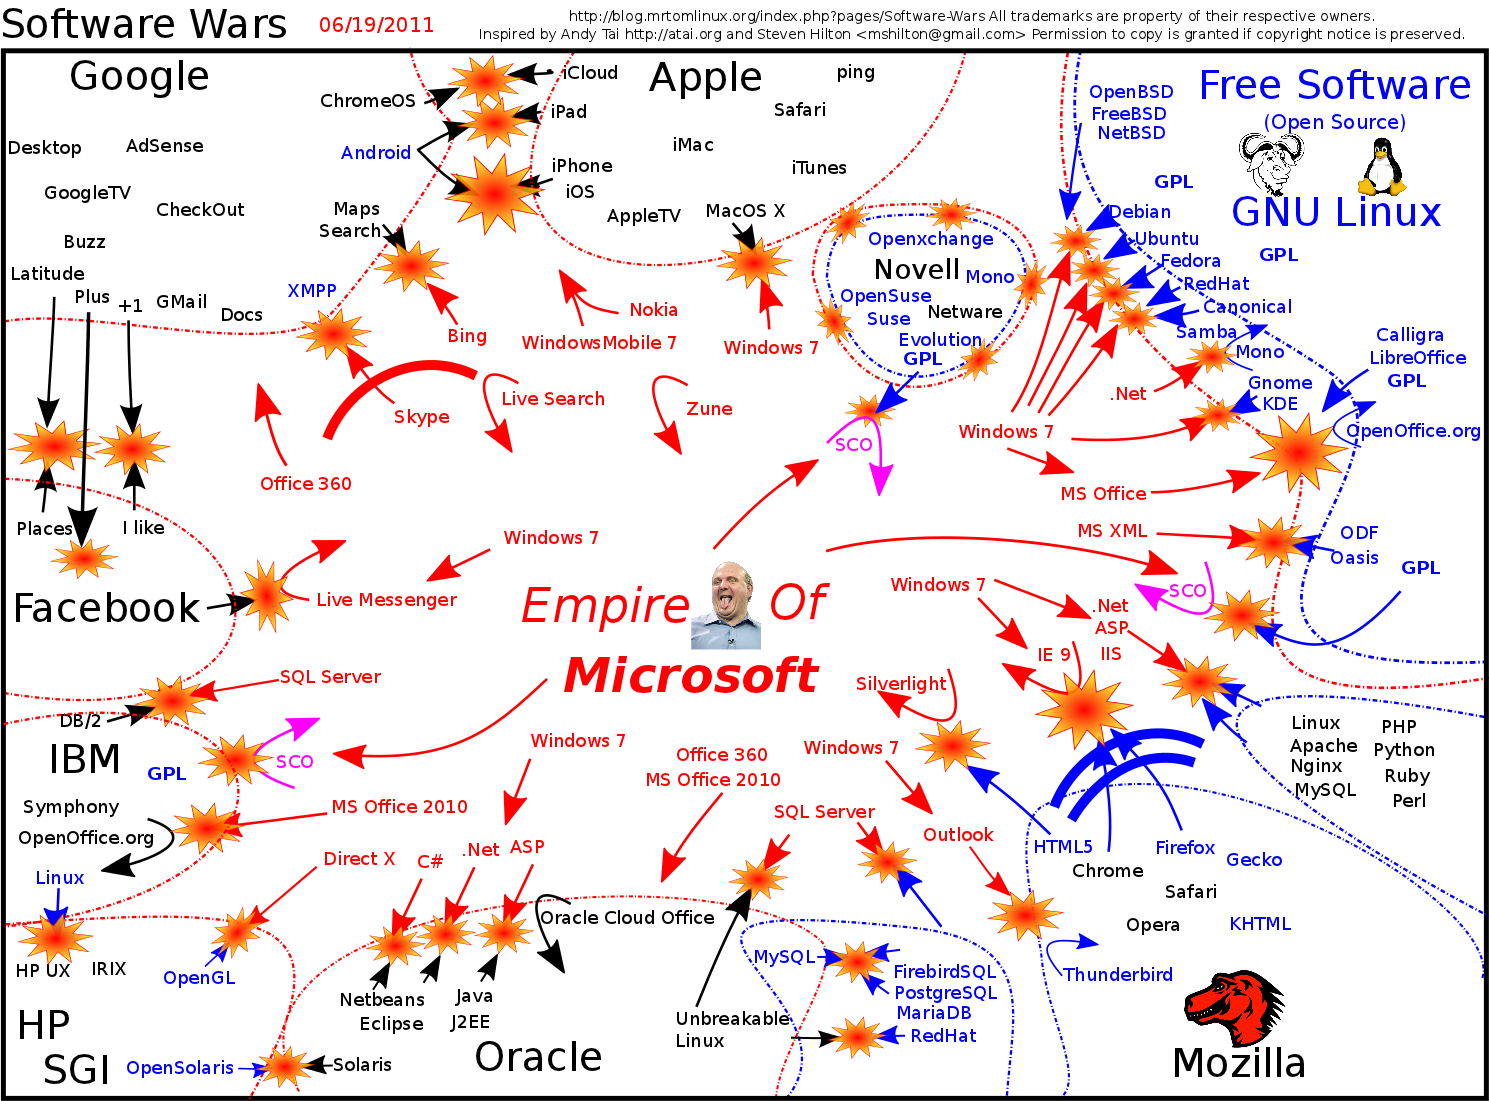
\includegraphics[width=0.9\linewidth]{slike/software_wars.png}
\end{center}
\end{frame}
%\subsection{Free as in free speech}


\section{Nekaj prednosti odprte kode}
\begin{frame}
\frametitle{Prednosti odprte kode}
\begin{enumerate}
\item U"cenje na primerih dobro napisanih programov
\item Varnost kode, ki jo preverja veliko prostovoljcev
\item Mo"znost spreminjanja delovanja programa
\item Je zanimiv poslovni model
\item "Vendor Lock-in" ni mogo"c (???)
\item Popolna svoboda, kako program uprabiti
\end{enumerate}
\begin{alert}{Pozor!}
Prosto programje/odprta koda ne zagotavlja brezpla"cnosti
\end{alert}
\end{frame}

\section{Odprtokodne licence}
\subsection{OSI priznane odprtokodne licence}

\begin{frame}
\frametitle{Odptokodne licence}
\begin{itemize}
\item 58 priznanih licenc
\item 9 je popularnih in pokrivajo skoraj vse potrebe
\item za izdajo programa pod licenco ni potrebno kontaktirati nikogar
\item BREZ PRILO"ZENE LICENCE se za program smatra, kot da je strogo zaprto licenciran
\item pravna praksa je "se v povojih
\item licence z ve"c omejitvami pove"cajo mo"znost kr"sitve
\item ve"c licenc za isti program?
\end{itemize}
\end{frame}

\subsection{Komercialno izkori"scanje odprtokodne programske opreme}

\begin{frame}
\begin{itemize}
\frametitle{Kako poslovno izkori"s"cati odprto kodo?}
\item "ce je koda odprta, je lahko produkt za"s"citen z blagovno znamko (Firefox vs. Iceweasel)
\item tekmeci lahko forkajo kodo, ne morejo pa blagovne znamke (OpenOffice vs. LibreOffice)
\item izobra"zevanja o uporabi va"sih programov ali drugih programov
\item prilagoditev programov posebnim "zeljam in potrebam stranke
\item svetovanje
\item podpora
\end{itemize}
\end{frame}
%\section{Uporabnik v svetu odprte kode}

\begin{frame}
\frametitle{Raz"sirjena Odprtokodna Programska orodja}
\begin{itemize}
\item \TeX in \LaTeX
\item Octave, Maxima, Python in numpy, R
\item Firefox, Thunderbird
\item OpenOffice, LibreOffice
\item GIT
\item Kicad
\item VLC, mplayer
\item BitTorrent
\item Inkscape
\item Gimp
\end{itemize}
\end{frame}

\section{Dru"zba in odprta koda}
\subsection{Odprta koda in trajnostni razvoj}
\begin{frame}
\frametitle{Javna uprava/javne slu"zbe}
\begin{itemize}
\item odprta koda je cenej"sa
\item prehod na odprto kodo ni brezpla"cen
\item prilagoditve odprtokodnih re"sitev pomeni zaslu"zek za doma"ce gospodarstvo
\item na podro"cju informatike odprta koda zaposluje doma"ci kader (zmanj"sanje brezposelnosti)
\item lobiji
\item problem odgovornosti (la"zna varnost?)
\end{itemize}
\end{frame}

\begin{frame}
\frametitle{Primer: Ob"cinska uprava M\"{u}nchen}
\begin{itemize}
\item za nadgradnjo OS Microsoft Windows bi porabili 34 miljonov evrov
\item prehod za"cnejo leta 2004
\item na Linux preide 14.800 uporabnikov
\item na OpenOffice preide 15.000 uporabnikov
\item za prehod na Linux in odprto kodo so porabili 23 miljonov evrov
\item (ve"cina denarja se je vrnila med doma"ce strokovnjake!) 
\end{itemize}
\end{frame}

\subsection{Informacije}

\begin{frame}
\frametitle{Javno dostopne informacije}
\begin{itemize}
\item Podatki financirani iz javnih sredstev pripadajo javnosti. Da ali ne?
\item Obstaja mno"zica javno dostopnih informacij pomembnih za razvoj dru"zbe, vendar je teh "se vedno premalo
\end{itemize}
\end{frame}

\begin{frame}
\frametitle{Primer: Arhiv dru"zboslovnih podatkov}
\begin{itemize}
\item ve"c kot 600 dru"zboslovnih raziskav "sir"sega pomena za raziskovalce 
\item s svojimi 16-letnimi izku"snjami pomagajo pri "sirjenju arhitekture za hranjenje podatkov (so edini tako ob"siren podatkovni arhiv v Sloveniji)
\item sodelujejo na projektu Odprti podatki -- predlog ravnanja z raziskovalnimi podatki vseh podro"cij
\item so odprti za sodelovanje z in"stitucijami za "sirjenje duha odprtih tehnologij, odprte kode in odprtih podatkov
\end{itemize}
\end{frame}

\begin{frame}
\frametitle{"Zvi"zga"ci}
\begin{itemize}
\item ``Information wants to be free'', parafraziran RMS.
\item kontroverzna problematika
\item NSA in vohunjenje
\item Dilema: Ali morajo biti vsi podatki, ki se dotikajo javnosti javni ali je bolje da so nekateri skriti?
\end{itemize}
\end{frame}

\subsection{Finance}
\begin{frame}
\frametitle{Bitcoin}
\begin{itemize}
\item temelji na matemati"cnih predpostavkah
\item decentralizirana kriptovaluta (ni bank)
\item prenosi so anonimni (problem pranja denarja?)
\item trn v peti Ameri"ski administraciji (nevarnost za dolar)
\item na tiho ga podpira Kitajska (nevarnost za dolar)
\item na borzah se je ustalil pri vrednosti okoli 400EUR/BTC
\item bitcoine lahko ``rudarimo'' sami
\item "stevilo bitcoinov je omejeno
\item so deljivi na 8 decimalnih mest
\item avtor bitcoina Satoshi Nakamoto je neznan (bolje zanj!)
\end{itemize}
\end{frame}

%\subsection{Politika}
%\begin{frame}
%\frametitle{Elektronsko glasovanje}
%\end{frame}
%\begin{frame}
%\frametitle{Neposredna demokracija}
%\end{frame}


\subsection{Odprta koda drugje}
\begin{frame}
\frametitle{Strojna oprema}
\begin{itemize}
\item Arduino
\item Raspberry Pi
\item OpenStack
\item OLPC project
\item OpenMoko
\item Nokia N900
\end{itemize}
\end{frame}

\begin{frame}
\frametitle{Kultura}
\begin{itemize}
\item Odprti filmi in risanke
\item Odprta glasba
\item Po poteku avtorskih pravic je vsa literatura javna dobrina. Knjige zbira Gutenberg project.
\end{itemize}
\end{frame}

\begin{frame}
\frametitle{Znanost in izobra"zevanje}
\begin{itemize}
\item Odprta baza raziskovalnih podatkov: openscience.org, ...
\item nekatere znanstvene revije ponujajo t.i. ``open access''
\item Odprta predavanja
\item Ra"cunalni"ska oprema v osnovnih in srednjih "solah
\end{itemize}
\end{frame}
\begin{frame}
\frametitle{Hrana in pija"ca}
\begin{itemize}
\item recepti so odprtokodna izmenjava informacij
\item Open Soda
\item Free Beer
\end{itemize}
\end{frame}

\begin{frame}
\frametitle{Zahvala sodelavcem}
Jernej Podlipnik, Damjan Sirnik, Jernej Sorta, Klemen Grm, O"zbolt Menegati, Urban Bevc, Eva "Segatin, Andra"z Brodnik, Ale"s Berkopec, Miha Fo"snari"c, Edi Buli\'{c}, Matej Rabzelj, Dejan Hrovatin, Borut Pe"car, Andrej Panger"ci"c, Miha Pirnat, Matja"z Tome, Primo"z Meku"c 
\end{frame}
\end{document}
